In \secref{prior_perturbations} we considered a multiplicative perturbations
of the form \eqref{phi_perturbation} with the $\norminf{\cdot}$ norm.  In
this section we consider other norms, illustrating that other choices
have problems with KL divergence.

First, we recall what we hope to get from our linear approximation.  We wish to
approximation $\etaopt(\phi)$ using the linear approximation $\etalin(\phi)$
evaluated at $\phiz$, hoping that the error $\norm{\etaopt(\phi) -
\etalin(\phi)}_2$ is small whenever the $\norm{\phi}$ is small (for some choice
of $\norm{\cdot}$).  A bare minimum for such a local approximation to work is
for $\phi \mapsto \etaopt(\phi)$ to be continuous, so that, for any
$\phi$,
%
\begin{align*}
%
\lim_{t \rightarrow 0} \norm{\etaopt(t \phi) - \etaopt}_2 = 0.
%
\end{align*}
%
By this reasoning, however, $\etaopt$ itself is a ``good'' approximation to
$\etaopt(\phi)$ when $\norm{\phi}$ is small---when $\phi$ is small, by
continuity we can simply say that nothing has changed and be reasonably correct.
From our linear approximation, we expect another order of accuracy, namely that
%
\begin{align*}
%
\lim_{t \rightarrow 0} \frac{\norm{\etaopt(t \phi) - \etalin(t\phi)}_2}{t} = 0.
%
\end{align*}
%
That is, we expect an extra order of accuracy from our linear approximation
in $\norm{\phi}$.

The preceding display is enough if we have a fixed $\phi$ in mind.  However, if
we want to search over a larger set of candidate $\phi$, we want the derivative
to provide a {\em uniformly good approximation} to $\etaopt(\phi)$ amonst some
set of $\phi$, say, all bounded $\phi: \norm{\phi} \le 1$.  One way of
formalizing the notion of ``uniformaly good approximation'' follows.

%%%%%%%%%%%%%%%%%%%%%%%%%%%%%%%%%%%%%%%%%%%%%%%%%%%%%%%%%%%%%%%%%%%%%%%%%%%
%%%%%%%%%%%%%%%%%%%%%%%%%%%%%%%%%%%%%%%%%%%%%%%%%%%%%%%%%%%%%%%%%%%%%%%%%%%
\begin{defn}\deflabel{diffable_classes}
    (\citep[Definition 4.5]{zeidler:2013:functional})
%
Let $B_1$ and $B_2$ denote Banach spaces, and let $\ball_1 \subseteq B_1$ define
an open neighborhood of $\phi_0 \in B_1$.  Fix a function $f: \ball_1
\mapsto B_2$.

The function $f$ is {\em directionally differentiable} (also known as a Gateaux
differentiable) if there exists a bounded linear functional $f^{\mathrm{lin}}:
B_1 \mapsto B_2$ such that
%
\begin{align*}
%
\textrm{For any }\phi: \norm{\phi - \phi_0} = 1\textrm{, }
\lim_{t \rightarrow 0}
    \frac{f(\phi) - f(\phi_0) -
          f^{\mathrm{lin}}(t (\phi - \phi_0) )
         }{t} \rightarrow 0.
%
\end{align*}
%

Similarly, the function $f$ is {\em boundedly differentiable} (also known as
Fr{\'echet} differentiable) at $\phi_0$ if
%
\begin{align*}
%
\lim_{t \rightarrow 0}
    \sup_{\phi: \norm{\phi - \phi_0} = 1}
    \frac{f(\phi) - f(\phi_0) -
          f^{\mathrm{lin}}(t (\phi - \phi_0))
         }{t} \rightarrow 0.
%
\end{align*}
%
\end{defn}
%%%%%%%%%%%%%%%%%%%%%%%%%%%%%%%%%%%%%%%%%%%%%%%%%%%%%%%%%%%%%%%%%%%%%%%%%%%

Note that we used the same notation $f^{\mathrm{lin}}$ for both derivatives in
\defref{diffable_classes}.  In fact, if a function is compactly differentiable
then the two derivatives must coincide \citep[Proposition
4.8]{zeidler:2013:functional}, which justifies our presumptuous notation.

The difference between bounded and directional differentiability is whether the
linear approximation holds uniformly in $\phi$.  It is possible for functions to
be directionally but not boundedly differentiable even in $\mathbb{R}^2$, as the
next example from \citet{averbukh:1967:theory} demonstrates.

%%%%%%%%%%%%%%%%%%%%%%%%%%%%%%%%%%%%%%%%%%%%%%%%%%%%%%%%%%%%%%%%%%%%%%%%%
%%%%%%%%%%%%%%%%%%%%%%%%%%%%%%%%%%%%%%%%%%%%%%%%%%%%%%%%%%%%%%%%%%%%%%%%%
\begin{ex}\exlabel{averbukh}
%
(\citet[Example 1.9]{averbukh:1967:theory})
%
Consider $(x_1, x_2) \in \mathbb{R}^2$ and the polar coordinates $r :=
\sqrt{x_1^2 + x_2^2}$ and $\theta := \arctan(x_2 / x_1)$.  Let $\{\pi k: k \in
\mathbb{Z} \}$ denote integer multiples of $\pi$.  Define
%
\begin{align*}
%
f(r, \theta) := \begin{cases}
\frac{r^2}{| \sin \theta |} \exp\left( -\frac{r}{|\sin \theta|}\right)
    & \textrm{when } \theta \notin \{\pi k: k \in \mathbb{Z} \} \\
0. & \textrm{when } \theta \in \{\pi k: k \in \mathbb{Z} \}
%
\end{cases}
%
\end{align*}
%
Then $f$ is continuous at $(0, 0)$ and has a directional derivative in every
direction, but is not Fr{\'e}chet differentiable.
%
\begin{proof}
%
It is easy to show that $\sup_{y \ge 0} y \exp(-y) = \exp(-1)$, which is
achieved at $y=1$. So, for any $(r_1, \theta_1)$ and $(r_2, \theta_2)$,
$\abs{f(r_1, \theta_1) - f(r_2, \theta_2)} \le \abs{r_1 - r_2} \exp(-1)$, from
which it follows that $f(r, \theta)$ is continuous at $0$.  Moreover, for any
fixed direction $\theta$, $\fracat{\partial f(r, \theta)}{\partial r}{r=0} = 0$,
so the linear approximation to $f(r, \theta)$ at $(0, 0)$ in any direction is
identically zero.  For any $r > 0$, the error in the linear approximation is
given by $\sup_{\theta} \abs{f(r, \theta) - 0} = r \exp(-1)$, which is achieved
by setting $r / |\sin \theta| = 1$.  Thus the error in the linear approximation
is of order $r$, not smaller.
%
\end{proof}
%
\end{ex}
%%%%%%%%%%%%%%%%%%%%%%%%%%%%%%%%%%%%%%%%%%%%%%%%%%%%%%%%%%%%%%%%%%%%%%%%%
%
%%%%%%%%%%%%%%%%%%%%%%%%%%%%%%%%%%%%%%%%%%%%%%%%%%%%%%%%%%%%%%%%%%%%%%%%%
%%%%%%%%%%%%%%%%%%%%%%%%%%%%%%%%%%%%%%%%%%%%%%%%%%%%%%%%%%%%%%%%%%%%%%%%%
\begin{figure}[h!]

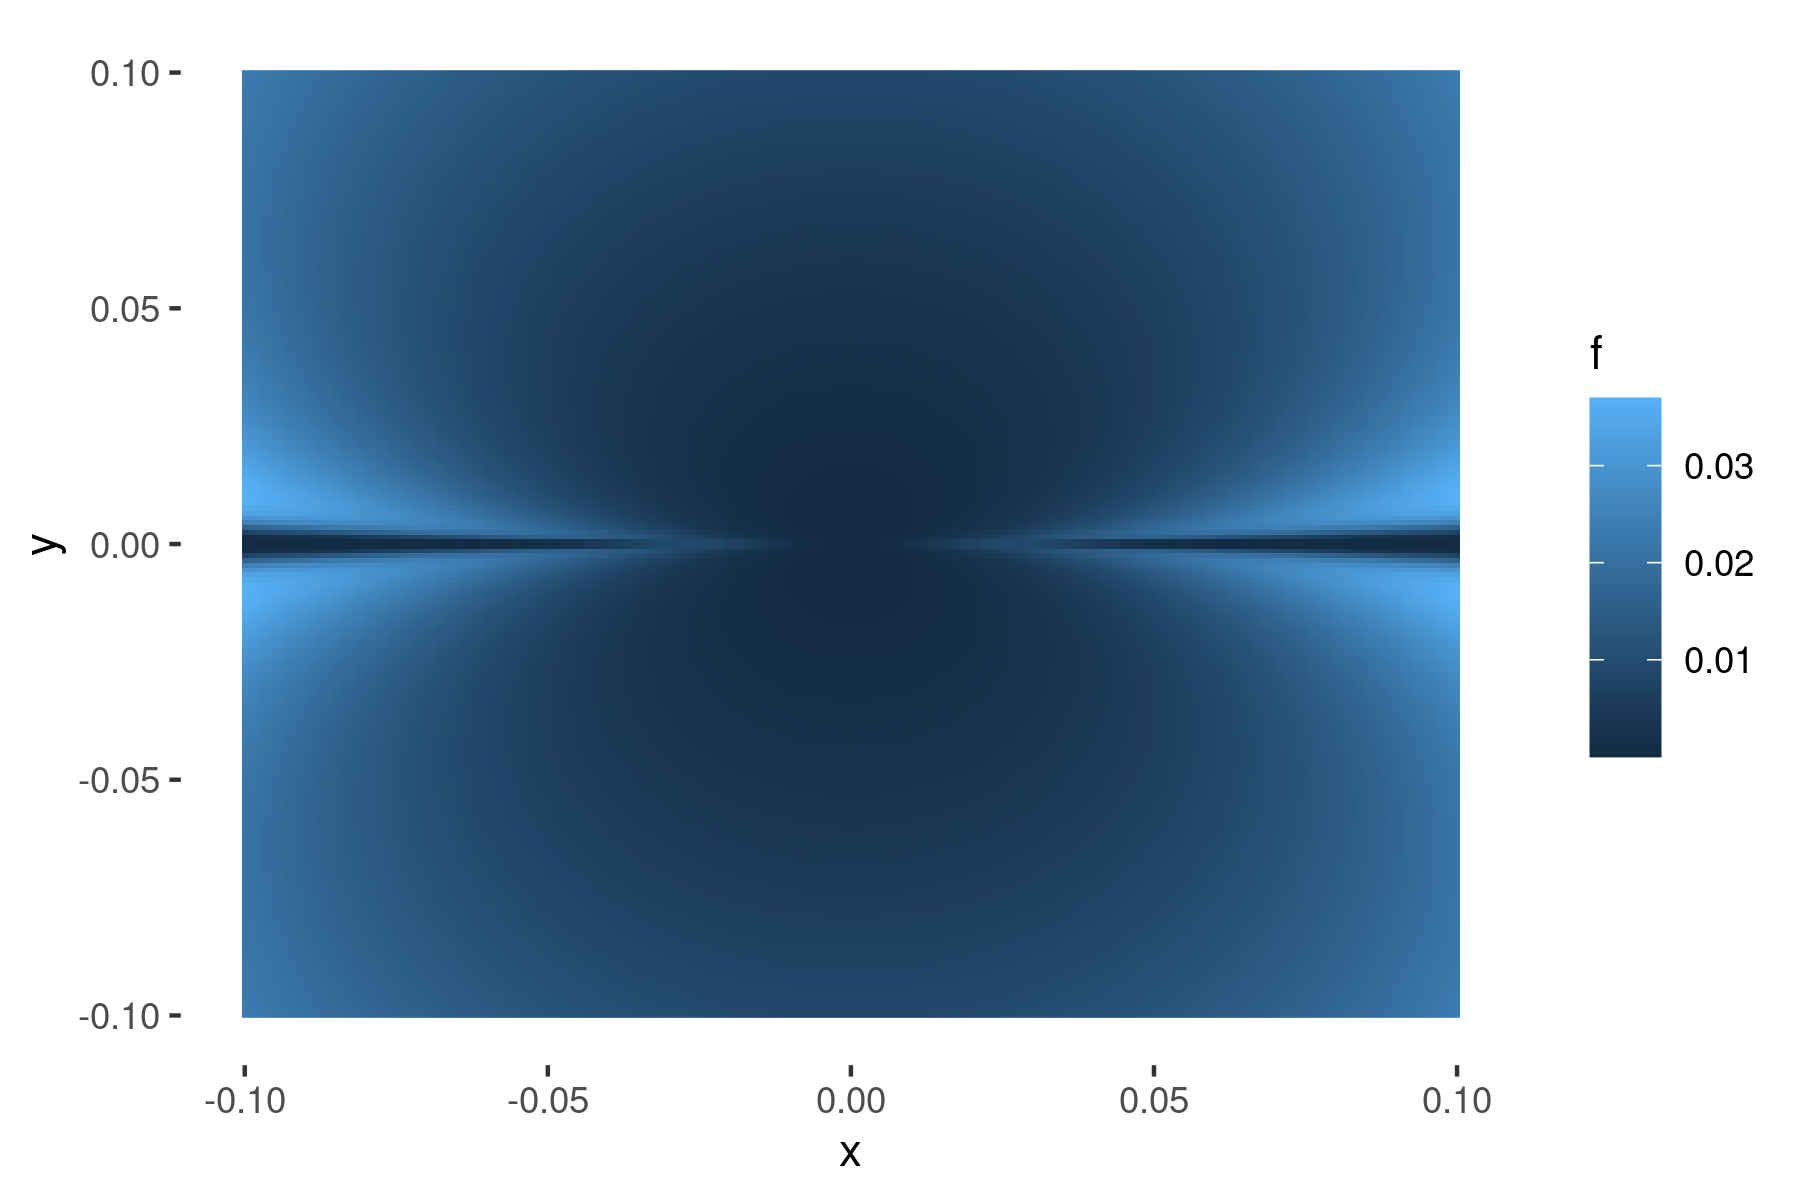
\includegraphics[width=0.980\linewidth,height=0.667\linewidth]{static_images/averbukh_example.png}
\caption{A plot of $f(x_1, x_2)$ from \exref{averbukh}.}\figlabel{averbukh_plot}
\centering
\end{figure}
%%%%%%%%%%%%%%%%%%%%%%%%%%%%%%%%%%%%%%%%%%%%%%%%%%%%%%%%%%%%%%%%%%%%%%%%%

See \figref{averbukh_plot} for a plot of \exref{averbukh}.  The function $f(r,
\theta)$ is sufficiently flat in neighborhood of $0$ that its best linear
approximation in any direction is identically $0$, so the directional
derivatives give no more information than using continuity. However, some
directions $\theta$ are worse than others, and which direction is worst depends
on $r$, in such a way that the function $f(r, \theta)$ actually approaches $0$
at the rate $r$.

One must go through special effort to construct functions that are
directionally but not boundedly differentiable in $\mathbb{R}^2$, but in
infinite dimensional Banach spaces it is easier.



-------------------

The above example is not the best.  What we want to say is that if a function is
Frechet differentiable then it is continuous.  (Zeidler Proposition 4.5 (d)). It
is possible to define discontinuous functions whose Gateaux derivatives exist.
And this is what we are worried about.  For this, a simpler R2 example will
suffice.  And we can use the function $\expect{\q(\theta)}{\log(1 +
\phi(\theta))}$ with the L2 norm as an example, which is perfect.
